% vim:encoding=utf8 ft=tex sts=2 sw=2 et:

\documentclass{classrep}
\usepackage[utf8]{inputenc}
\usepackage{graphicx}

\studycycle{Informatyka, studia dzienne, mgr jednolite}
\coursesemester{IX}

\coursename{Obliczenia ewolucyjne}
\courseyear{2010/2011}

\courseteacher{mgr inż. Łukasz Chomątek}
\coursegroup{wtorek, 14:15}

\author{
  \studentinfo{Cezar Pokorski}{138077} \and
  \studentinfo{Artur Czajka}{137971} 
}

\title{Zadanie 3: Ewolucyjna optymalizacja kształtu na przykładzie brachistochrony}
\svnurl{[Mercurial]https://aelabnull.googlecode.com/hg/}

\begin{document}
\maketitle

\section{Opis zadania}
Należy pokazać, ze brachistochrona jest łukiem cykloidy stosując np.~strategie
ewolucyjne. Można wykorzystac funkcje sklejane (punkty kontrolne - zalecane) 
lub wielomiany aproksymacyjne.

\textbf{Brachistochrona} to krzywa, po której czas staczania się masy punktowej od~punktu~A
do~punktu~B pod wpływem stałej siły (siły ciężkości) jest najkrótszy. 



\section{Implementacja}
Do rozwiązania tego zadania posłużyliśmy się językiem Python oraz pakietami \texttt{matplotlib} 
i~\texttt{numpy}. 

\subsection{Reprezentacja}
Jako podstawę rozwiązania utworzyliśmy klasę \texttt{Bezier} --- jej obiekty reprezentują
krzywe Beziéra, stanowiące osobniki naszej populacji. Każda z~takich krzywych posiada cztery
punkty charakterystyczne, $p_{0..3}$, jednoznacznie opisujące jej kształt. Do~rozwiązania
problemu przedstawionego w~tym zadaniu przyjmujemy wręcz, że punkty $p_0$ oraz $p_3$ są~ustalone
jako początkowy i~końcowy punkt pewnego badanego spadku, mają zatem współrzędne $p_0 = A = (0, Y)$,
$p_3 = B = (X, 0)$, gdzie $X$ umownie rozumiemy jako szerokość wykresu, $Y$ zaś jako jego wysokość 
(jest to wysokość, z~której stacza się ciało). Drogę pomiędzy nimi wytycza kształt krzywej.

Całość procesu polega zatem na~wykorzystaniu strategii ewolucyjnej w~celu takiej optymalizacji
punktów $p_1$ i~$p_2$ aby czas staczania się masy punktowej był najkrótszy.  Punkty te opisane~są 
za~pomocą wektorów współrzędnych rzeczywistych (typu \texttt{numpy.array}) zawierających ich
współrzędne. Ich początkowe wartości dobierane są~losowo z przedziału $x\in(0,X), y\in(-Y,Y)$.

Na populację składa się pewna liczba $N$ (domyślnie 40) osobników, każdy z~nich jest pojedynczą
krzywą Beziéra. Dla każdego osobnika obliczana jest jego "jakość" jako czas potrzebny do~pokonania
wyznacoznej przez~nią trasy, gdzie najniższy czas oznacza wynik najlepszy (najlepsze przystosowanie).

\subsection{Operatory krzyżowania i mutacji}
Ponieważ osobniki kodowane są~jako zestawienia (czterech) współrzednych rzeczywistych, 
operator krzyżowania zdefiniowany jest jako średnia ważona współrzędnych obojga rodziców. 
Każde krzyżowanie generuje dwóch potomków, z~których jeden przyjmuje cechy jednego rodzica
z~wagą~0.3, a~drugiego z~wagą 0.7, drugi zaś -- odwrotnie. Nic nie stoi na~przeszkodzie 
by~zmodyfikować te parametry, jednak w~praktyce okazują się dostatecznie dobre (a~na~pewno
bardziej interesujące od średniej arytmetycznej i~pojedynczego potomka), a~operator krzyżowania
oparty o~średnią generalnie i~tak odgrywa mniejszą rolę, gdyż bardzo ważny staje się operator
mutacji.

Mutacja przebiega następująco: wybierana jest losowo jedna z~czterech $(p_{1_x}, p_{1_y}, p_{2_x}, p_{2_y})$
współrzędnych, która zostanie poddana modyfikacji, następnie zaś modyfikowana jest o~wartość
z~przedziału odpowiednio $(-\frac{1}{4}{X}, \frac{1}{4}{X})$ lub $(-\frac{1}{4}{Y}, \frac{1}{4}{Y})$,
dobraną losowo z~rozkładem jednostajnym. Chociaż powoduje to~stosunkowo duże modyfikacje, są~one tutaj
bardzo pożądane i~wprowadzają element "eksperymentu" i~"świezości", zapobiegając stagnacji algorytmu.


\subsection{Ocena przystosowania}

Aby ocenić przystosowanie osobnika, obliczamy przybliżony "czas" staczania masy punktowej 
wzdłuż wyznaczonej przez niego krzywej. Obliczenia~te nie~muszą być wysoce precyzyjne, ważne
natomiast by~pozwalały porównywać osobniki i~odzwierciedlały charakter zjawiska, które niejako
modelują.

Dla każdego osobnika próbkujemy krzywą dzieląc ją na pewną ilość równych\footnote{równych tak naprawdę
nie w~sensie współrzędnej $x$ a~raczej parametru $t$ we~wzorze $p(t)=\sum_{i=0}^{n}{p_i B_i^n(t)}$, 
$t\in[0,1]$ opisującym wszystkie współrzędne punktu na~krzywej. Są~to~zatem przedziały o~równej 
długości krzywej, a~nie równo odległe w~$x$.} przedziałów. 

W~każdym z~nich zaś obliczamy przyspieszenie $a$ wynikające z~działania siły grawitacji na~ciało, 
przy czym każdy taki odcinek traktujemy jak małą równię pochyłą, gdzie $a=g\frac{h}{l}$ 
($h$ -- wysokość, z~której masa opada, $l$ -- długość odcinka, jaki~przebywa).

Znając $a$ w danym kroku, uaktualniamy prędkość ciała $v$ i~sprawdzamy, czy nie doszło do~zatrzymania
lub wręcz cofania się ciała (gdy $v \leq 0$, stwierdzamy, że~ciało nie stoczy~się nigdy i~jako
czas staczania zwracamy nieskończoność (\texttt{numpy.inf})). Pozwala to~wykryć krzywe, które nie~
miałyby sensu fizycznego.

Po~posortowaniu osobników od najlepszego do najgorszego dokonujemy standardowego krzyżowania 
osobników dopasowanych najlepiej oraz przeprowadzamy ewentualne mutacje, uwzględniając przy tym oczywiście
parametry takie, jak~prawdopodobieństwo krzyżowania i~prawdopodobieństwo mutacji. \\

Podczas pracy programu można obserwować kształt najlepszej uzyskanej w~danej epoce krzywej.

\section {Wyniki i wnioski}
Końcowym rezultatem działania algorytmu jest zwykle krzywa o~poniższym wyglądzie:
\begin{center}
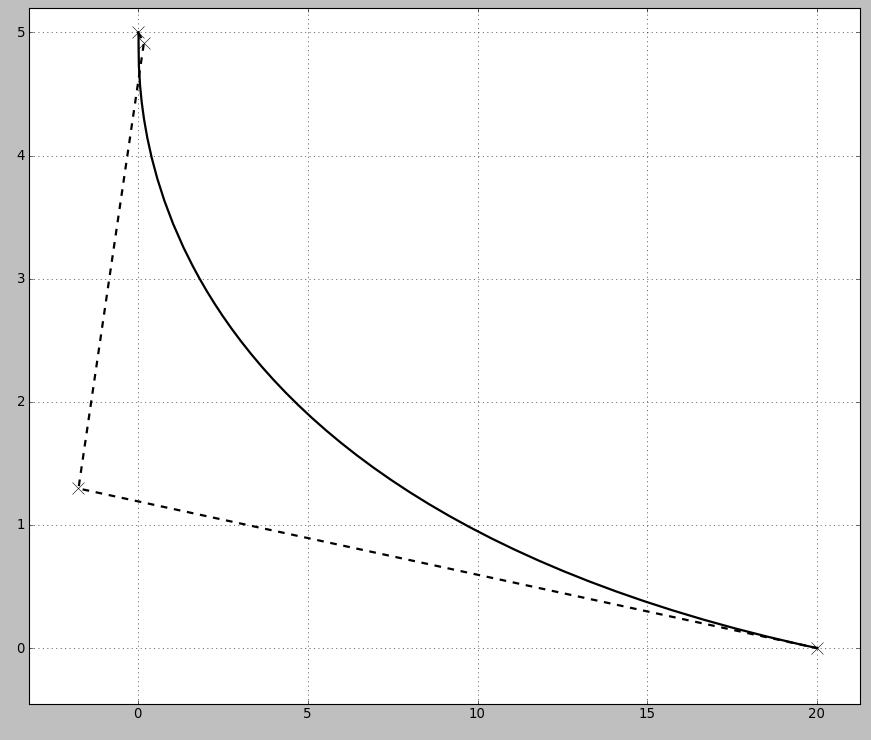
\includegraphics[scale=0.30]{screenshot7.png}
\end{center}
Za każdym przebiegiem algorytmu zauważamy, że:
\begin{itemize}
  \item punkt $p_1$ praktycznie redukuje się do punktu $p_0$ w pierwszych iteracjach. Wynika z~tego, że~taką krzywą można równie skutecznie reprezentować za~pomocą jednego tylko punktu charakterystycznego.
  \item za każdym razem efektem jest krzywa, której początkowy fragment jest "bardziej pionowy", dalej zaś krzywa zbiega do~linii prostej. W~poczatkowej fazie ruchu nasze ciało nabiera zatem prędkości, która pozwala mu przebyć pozostałą część drogi po~trasie bliskiej najkrótszej euklidesowej trasie między tymi punktami.
  \item w~zadaniu tym zwiększenie pradopodobieństwa mutacji pomaga programowi szybciej odnaleźć optymalny kształt krzywej, mimo zaburzeń wprowadzanych przez mutację. Nawet dla prawdopodobieństwa mutacji wynoszącego $P_{mutacji}=1$ program dąży do podobnego rozwiązania. Zbyt mała mutacja powoduje zaś szybkie uśrednienie wszystkich osobników populacji i~zanik różnorodności --- a~zatem i~eksplorowania nowych rozwiązań.
\end{itemize}

\end{document}
